% arara: pdflatex: {synctex: yes, action: nonstopmode}
% arara: pdflatex 
% arara: bibtex 
% arara: pdflatex
% arara: pdflatex
% arara: nomencl
% arara: pdflatex: {synctex: yes, action: nonstopmode}

%\documentclass[a4crop]{ntnuthesis} 
\documentclass{ntnuthesis}  
\usepackage{amsmath} %equations and spacings
\usepackage[utf8]{inputenc}
\usepackage{lipsum} % acces to random text
%graphics
\usepackage{graphicx}
%\usepackage[demo]{graphicx}
%caption styles
\usepackage[small,bf]{caption}
%\usepackage{caption}
\usepackage[labelformat=simple]{subcaption}
\renewcommand\thesubfigure{(\alph{subfigure})} % see subcaption doc
%<<byman 
\usepackage{colortbl}
\usepackage{xcolor}
\usepackage{color}
\usepackage{sidecap}
%byman>>

\usepackage{listings}
\usepackage{color} %red, green, blue, yellow, cyan, magenta, black, white
\definecolor{mygreen}{RGB}{28,172,0} % color values Red, Green, Blue
\definecolor{mylilas}{RGB}{170,55,241}

%<<byman
%% We want UK-english hyphenation patterns.byman
\usepackage[british]{babel}
%byman>>

%Remove Paragraph indenting
\setlength{\parindent}{0.0in} 
\setlength{\parskip}{0.1in}

%<<byman
%% Use scalable, PostScript Type 1 versions of the Computer Modern fonts.
\usepackage{type1cm}
%% Replace the standard Computer Modern Typewriter font LaTeX uses
%% for monospace text with the PostScript font Adobe Courier.
\usepackage{courier}
\usepackage[T1]{fontenc}
\usepackage{ae,aecompl}
\usepackage{times}
%% Redefine the font used for the section headings to
%% Helvetica-Narrow Bold.
\usepackage{sectsty}
\allsectionsfont{\usefont{OT1}{phv}{bc}{n}\selectfont}
% for colour shades in tables 
\usepackage{colortbl} 
 %to control the title formating and spaces around the titles
 \usepackage{pdfpages}
\usepackage[compact]{titlesec}
%%byman>>


%spaces under sections
\usepackage[compact]{titlesec}
\titlespacing{\section}{0pt}{*0}{*0}
\titlespacing{\subsection}{0pt}{*0}{*0}
\titlespacing{\subsubsection}{0pt}{*0}{*0}
%fonts
 %\usepackage[T1]{fontenc} %gives light font
 %\usepackage[light,math]{iwona}

%Abbreviations or Acronyms
%\usepackage[intoc]{nomencl}
\usepackage{nomencl}
\renewcommand{\nomname}{List of Abbreviations}
\makenomenclature

%Bibliography
%\usepackage{url}
\usepackage[]{natbib}%\usepackage[sectionbib]{natbib}
\usepackage{chapterbib}
%\bibpunct[:]{(}{)}{;}{a}{}{,} %citation structure
%\bibpunct{(}{)}{,}{a}{}{;} 
%\bibpunct{[}{]}{,}{a}{}{;}
%\bibpunct{(}{)}{;}{a}{}{,} % to follow the A&A style
%\usepackage{chapterbib}
\usepackage{hyperref}
%\hypersetup{colorlinks=true,citecolor=blue}
\hypersetup{colorlinks=true,citecolor=blue,linkcolor=blue,urlcolor=blue}

%To change box color around the links and citations, you have these other options :
%\hypersetup{citebordercolor=Violet,filebordercolor=Red,linkbordercolor=Blue}

\newcommand{\cmt}[1]{}%inline comment
  
%tabularx
\usepackage{tabularx}
\usepackage{tabulary}
\usepackage{longtable} %table on several pages
\usepackage{booktabs}

%enumerate(control spacing)
\newenvironment{packed_enum}{
\begin{enumerate}
	\vspace*{-1}
  	\setlength{\itemsep}{1pt}
  	\setlength{\parskip}{0pt}
  	\setlength{\parsep}{0pt}
}{\end{enumerate}}

%<<byman
\usepackage{multirow}
\usepackage{dcolumn}
\newcolumntype{d}{D{.}{.}{-2}}
\newcommand{\tabincell}[1]{\begin{tabular}{c}#1\end{tabular}}
\newcommand{\tabincellt}[1]{\begin{tabular}{l}#1\end{tabular}}
\newcommand{\merge}[1]{\multicolumn{1}{c}{#1}}

\usepackage{array}
\newcommand{\PreserveBackslash}[1]{\let\temp=\\#1\let\\=\temp}
\newcolumntype{C}[1]{>{\PreserveBackslash\centering}p{#1}}
\newcolumntype{R}[1]{>{\PreserveBackslash\raggedleft}p{#1}}
\newcolumntype{L}[1]{>{\PreserveBackslash\raggedright}p{#1}}

% Used to create tables with rows/cols spanning over se
%% Use fancy chapter headers, with Jos Dingjan's modifications,
%% plus my own tweaks. This style is not part of teTeX,
%% so we are using a local (and renamed) copy.
%\usepackage[Lenny]{fncychapleo}
\usepackage{fncychap}

%% Nicely format and linebreak URLs in the bibliography (and elsewhere).
%%\usepackage{url}
%% Define a new 'leo' style for the package that will use a smaller font.
\makeatletter
\def\url@leostyle{%
  \@ifundefined{selectfont}{\def\UrlFont{\sf}}{\def\UrlFont{\small\ttfamily}}}
\makeatother
%% Now actually use the newly defined style.
\urlstyle{leo}
%byman>>

%graphics
\usepackage{epstopdf} %support for eps.
\DeclareGraphicsExtensions{.eps,.ps,.pdf,.png,.jpg}
\usepackage{float} % figure placing [H]

%landscape Option
\usepackage{lscape} %Left down
%usepackage{pdflscape} %Left up)

\usepackage[draft]{todonotes}   % notes showed (JJUNJU)
% Select what to do with command \comment:  
% \newcommand{\comment}[1]{}  %comment not showed
\newcommand{\comment}[1]
{\par {\bfseries \color{red} #1 \par}} %comment showed

%Section Numbering and TOC depth
\setcounter{secnumdepth}{2}
\setcounter{tocdepth}{3}

%chapter biblio
\usepackage{chapterbib}


\usepackage{tikz-timing}
\usepackage{todonotes}
\usepackage{cleveref}

%Drawing flow charts
\usepackage{tikz}
\usetikzlibrary{shapes,arrows,arrows.meta,quotes}
\tikzstyle{decision} = [diamond, draw, fill=blue!20, 
    text width=4.5em, text badly centered, node distance=3cm, inner sep=0pt]
\tikzstyle{process} = [rectangle, draw, fill=blue!20, 
    text width=5em, text centered, rounded corners, minimum height=4em]
\tikzstyle{line} = [draw, -latex']
\tikzstyle{output} = [trapezium,draw, trapezium left angle=70,trapezium right angle=-70,fill=pink, text width=3em, minimum height=2em,text centered]
\tikzstyle{data} = [trapezium,draw, trapezium left angle=70,trapezium right angle=-70,fill=white!20, text width=3em, minimum height=2em,text centered]
\tikzstyle{space} = [rectangle, fill=white,opacity=0,text width=5em, text centered, rounded corners, minimum height=4em]
\tikzstyle{results} = [ellipse,draw,fill=white, text width=4em, minimum height=3em,text centered]

%To generate list of symbols
\newcommand{\addsymbol}[3]{%
  \symboldisplay{#1}{#2}\\%
  \setelem{#3}{#1}
}
\newcommand{\symboldisplay}[2]{%
  $#1$ \parbox{5in}{\dotfill #2}%
  %$#1$ \parbox{5in}{ #2}%
}
%\def\setelem#1{\expandafter\def\csname myarray(#1)\endcsname}
\def\setelem#1{\expandafter\gdef\csname myarray(#1)\endcsname}
\def\dispsymbol#1{\csname myarray(#1)\endcsname} 

%Titles
\title{Analysis of design parameters in a musical dual resonant solid state tesla coil}
%\subtitle{Subtitle of the thesis here}
\author{Øystein Smith}

\def \thesisAuthor{Øystein Smith}

%\degreetype{PhD}
\faculty{Faculty of Information Technology and Electrical Engineering}
\department{Department of Electronic Systems}
\copyrightnotice{All rights reserved}
\isbnprinted{}
\isbnelectronic{}
\serialnumber{}
\setyear{2017}
\setmonth{June}

\begin{document}

\frontmatter
\maketitle

%<<byman
%% Configuration of the header strings for the frontmatter pages.
\fancyhead[RO]{{\footnotesize\rightmark}\hspace{1em}\thepage}
\setcounter{tocdepth}{2}
\fancyhead[LE]{\thepage\hspace{1em}\footnotesize{\leftmark}}
\fancyhead[RE,LO]{}
\fancyhead[RO]{{\footnotesize\rightmark}\hspace{1em}\thepage}
%byman>>

\setcounter{page}{1}
\section*{Abstract}
Universities, science centers and other institutions has the need for equipment that demonstrates physical phenomena in interesting and audience friendly ways. An example of this is a Double Resonant Solid State Tesla Coil (DRSSTC). There is no big commercial or academic community for tesla coils, but tesla coils are mostly designed and used as a hobby. There are a few people sharing their designs on the internet that most of the tesla coil designs are based on. Few or none of these substantiate design choices or assumptions with physics and math. This thesis will attempt to substantiate the design choices done in the driver for a musical dual resonant solid state tesla coil.

This thesis discusses an implementation of a DRSSTC, substantiates the functionality of sub circuits and components with mathematics. Then discusses the mathematical description of the resonant transformer, varying component sizes, plotting and simulating the transfer functions. Then presents some measurements done on a physical implemented DRSSTC.

The component values or parameters that need to be adapted to the resonant frequency are; the delay in the latch reset network in the interrupter, the phase lead time in the interrupter, and the corner frequency of the noise filter in the limiter. The component values or parameters that need to be adapted to the current flowing in the primary resonant circuit are; the impedance of the feedback load in the interrupter and in the limiter, and the number of turns on the current feedback transformers.

In the resonant circuit we have proven that the ohmic resistances in both the primary and secondary circuit should be as small as possible to give a high as possible amplitude on the output, the conductance of the streamer does not seem to affect the resonant frequency (detuning) or the amplitude on the output, but does affect the current in the primary resonant circuit. And will affect the feedback signals. The coupling coefficient only affects the amplitude on the output, as long as no arcing happens between the primary and secondary coils. According to the transfer functions varying the capacitors or inductors does not give the same results as expected from the common assumptions in the hobby community. Here no other conclusions can be drawn other that this may be a topic for further research.

\newpage
\section*{Sammendrag}
Universiteter, vitenskapssentre og andre institusjoner har behov for utstyr som demonstrerer fysiske fenomener på interessante og publikumsvennlige måter. Et eksempel på dette er en Double Resonant Solid State Tesla Coil (DRSSTC). Det er ikke stort kommersielt eller faglig samfunn for tesla-spoler, men tesla-spoler er for det meste utformet og brukt som en hobby. Det er noen få personer som deler design på internett som de fleste av tesla-spolens design er basert på. Få eller ingen av disse underbygger designvalg eller antagelser med fysikk og matte. Denne oppgaven vil forsøke å underbygge designvalgene som er gjort i sjåføren for en musikalsk dual resonant solid state tesla coil.

Denne oppgaven diskuterer en implementering av et DRSSTC, underbygger funksjonaliteten til underkretser og komponenter med matematikk. Deretter diskuteres den matematiske beskrivelsen av resonanttransformatoren, varierende komponentstørrelser, plotting og simulering av overføringsfunksjonene. Deretter presenteres noen målinger gjort på en fysisk implementert DRSSTC.

Komponentverdiene eller parametrene som må tilpasses resonansfrekvensen er; Forsinkelsen i sperreinnstillingsnettverket i avbryteren, faseovergangstiden i avbryteren og hjørnefrekvensen av støyfilteret i begrenseren. Komponentverdiene eller parametrene som må tilpasses til strømmen som strømmer i den primære resonanskrets er; Impedansen til tilbakekoblingsbelastningen i avbryteren og i begrenseren, og antall svinger på gjeldende tilbakekoblingstransformatorer.

I resonanskretsen har vi bevist at de ohmiske motstandene i både primær- og sekundærkretsen bør være så små som mulig for å gi en høy som mulig amplitude på utgangen, synes ikke strømmen av strømmen til å påvirke resonansfrekvensen (detuning ) Eller amplitude på utgangen, men påvirker strømmen i den primære resonanskretsen. Og vil påvirke tilbakemeldingssignalene. Koblingskoeffisienten påvirker bare amplituden på utgangen, så lenge det ikke skjer noen bue mellom primær- og sekundærspolene. I henhold til overføringsfunksjonene varierer kondensatorene eller induktørene ikke med de samme resultatene som forventet fra de felles antagelsene i hobbyområdet. Her kan det ikke trekkes andre konklusjoner om at dette kan være et tema for videre forskning.
\newpage
\newpage
\section*{Preface}

Omega Verksted has a long tradition with providing Tesla Coil shows for the line union 'Omega' and for other student societies at NTNU. The current implementation is based on some inadequate documentation from the 2009 implementation. The 2009 implementation was in use up to 2014 and was notorious for blowing output transistors. As well as for being put together with hot glue. In 2014 an effort was begun to improve the reliability and portability of the tesla coil. A new implementation was created with the design split into modules to ease the further development. The connectors and the casing for the driver was replaced and a back plane architecture was selected improving portability and reliability greatly. And a project report was written on the back plane architecture \citep{prosjektoppgave}. The coil rig was also replaced as it had the tendency to catch fire. The mode of operation for this implementation of a DRSSTC or general DRSSTC implementations are still not understood fully by all members of the project. This thesis aims do provide adequate documentation on the current DRSSTC implementation at Omega Verksted. And to serve as an educational document to give project members the knowledge to change or improve on the implementation.

Thanks should be made to Omega Verksted who has financed the parts used for this project, Tim Cato Nedland at the department of acoustics who did the acoustic measurements, the department of electrical power engineering who provided a safe location to do measurements, and HSE coordinator Sverre Vegard Pettersen who helped to make it feasible to do safe measurements. Lastly thanks should be made to my supervisor Lars Lundheim who have provided invaluable support and guidance through the work on this thesis.
\cleardoublepage

%TOC
\tableofcontents
%\addcontentsline{toc}{chapter}{Contents}
\cleardoublepage

\listoftables	
\addcontentsline{toc}{chapter}{List of Tables}
\cleardoublepage

\listoffigures	
\addcontentsline{toc}{chapter}{List of Figures}
\cleardoublepage

%Abbreviations
%\newpage
%\thispagestyle{empty}
%\printnomenclature
%\cleardoublepage

%Symbols
%\newpage
%\chapter*{List of Symbols\hfill} 
%\addcontentsline{toc}{chapter}{List of Symbols}
%\begin{flushleft}
	%%\addsymbol{Driver}{Electronics for supplying signal and power to a coil rig forming a tesla coil}{}
%\addsymbol{Coil rig}{Coil inductors and capacitors forming a resonant circuit in the arrangement of a resonant transformer}{}
%\addsymbol{Primary resonant circuit}{The Coil inductor and capacitor on the primary side of the resonant transformer in a coil rig}{}
%\addsymbol{Secondary resonant circuit}{The Coil inductor and capacitor on the secondary side of the resonant transformer in a coil rig}{}

\textbf{Driver:} Electronics for supplying signal and power to a coil rig forming a tesla coil.

\textbf{Coil rig:} Coil inductors and capacitors forming a resonant circuit in the arrangement of a resonant transformer.

\textbf{Primary resonant circuit:} The Coil inductor and capacitor on the primary side of the resonant transformer in a coil rig.

\textbf{Secondary resonant circuit:} The Coil inductor and capacitor on the secondary side of the resonant transformer in a coil rig.

%\end{flushleft}

\mainmatter

\cleardoublepage
%\input{F01-copyright}
%\input{F02-dedication}

%\input{F05-acknowledgements}
%
%Chapters
%Introduksjon
\chapter{Introduction}
\label{intro}
Universities, science centers and other institutions has the need for equipment that demonstrates physical phenomena in interesting and audience friendly ways. An example of this is a Double Resonant Solid State Tesla Coil (DRSSTC). This is a contraption that by the use of high voltage generates a sequence of electrical discharges. When these discharges happen in air a sound wave is generated. By modulating the frequencies of these discharges one can generate sound with different tones. A DRSSTC can in this way be made into a musical instrument.
There is no big commercial or academic community for tesla coils, but tesla coils are mostly designed and used as a hobby. There are a few people sharing their designs on the internet that most of the tesla coil designs are based on. Few or none of these substantiate design choices or assumptions with physics and math. This thesis will attempt to substantiate the design choices done in the driver for a musical dual resonant solid state tesla coil.

\Cref{fig:teslabano} shows a DRSSTC in use where a streamer has formed from the top load to a grounded copper object.

\begin{figure}[ht]
    \centering
    \includegraphics[width=0.6\textwidth]{img/teslabano.jpg}
    \caption{A tesla coil in use}
    Photo: Sindre Vaskinn Hunn
    \label{fig:teslabano}
\end{figure}

\section{Tesla Coil}
\label{tesla}
%http://www.tfcbooks.com/tesla/contents.htm
The Tesla Coil is a form of resonant transformer invented by Nikolai Tesla and used for experiments with artificial illumination \citep{5570149}. A resonant transformer consists of two inductively coupled coils, each loaded with a capacitance such that they get the same resonance frequencies. The resonant transformer has since gotten a lot of applications, among others; RFID, NFC, and Wireless charging. The resonant transformer in the form of the Tesla Coil has also become a popular entertainment device.
%Death ray
%Entertainment

\section{Earlier work}
%Who has done work on this before? steve4hv, pupman, scantesla, loneoceans.
Some of the people who have done work on DRSSTC in the hobbby community are; Steve Ward \Citep{stevehv}, Jimmy Hynes \Citep{chunkyboy86}, Terry Fritz \Citep{terrel}, Steve Conner \Citep{conner}, Dan McCauley \Citep{easternvoltage}, and the tesla coil mailing list \Citep{pupman}. Among these there are few disagreements on how a tesla coil should be designed, there are few variations on the resonant circuit, but slightly more variation on the low voltage controlling side. Some use a preset oscillator to drive the resonant circuit, while others use feedback from either the primary or secondary resonant circuits.

There has been developed an drsstc tesla coil driver by Steve Ward witch other people have designed variations on \Citep{ud27}.

Simulation software for the resonant circuitry of tesla coils called Scantesla have been written \Citep{scantesla}.

Guidelines for the design of the resonant circuits can be found at most of the above mentioned sites.

A modular back plane based tesla coil driver implementation have been designed and implemented by the author together with other members of Omega Verksted\footnote{Omega Verksted is a association of electronics and hobby interested students at the Norwegian University of Science and Technology (NTNU) founded in 1971.}. This is based on earlier designs by members of Omega Verksted, the last major implementation at Omega Verksted was done in 2009 mostly by Dewald de Bruyn.

%Onetesla sells commercially

%Tables for coil aspect ratios.

%Beskrivelse av Tesla Coil / DRSSTC
%\section{Tesla Coil}
\label{tesla}
%http://www.tfcbooks.com/tesla/contents.htm
The Tesla Coil is a form of resonant transformer invented by Nikolai Tesla and used for experiments with artificial illumination \citep{5570149}. A resonant transformer consists of two inductively coupled coils, each loaded with a capacitance such that they get the same resonance frequencies. The resonant transformer has since gotten a lot of applications, among others; RFID, NFC, and Wireless charging. The resonant transformer in the form of the Tesla Coil has also become a popular entertainment device.
%Death ray
%Entertainment
%Tidligere arbeid
%\section{Earlier work}
Who has done work on this before? steve4hv, pupman, scantesla, loneoceans.
%Teori? nei
%\chapter{Theory}
What do you need to know to read this report.
%\section{Audio}

The audio produced by a musical tesla coil is distinctive and subjectively easily distinguished from the sounds produces by other musical instruments. The reason for this is that different musical instruments produce different harmonics (or overtones) based on different parameters in the instrument. In musical terms this is called timbre.

\subsection{Harmonics}

\subsection{Envelope}

\subsection{Timbre}
T

\subsection{Psychoacoustics}
Psychoacoustics is the scientific study of sound perception.


%Klang
%Overtoner
%Subjektivt

%Beskrivelse av arkitektur (Blokkoppbygning)
\chapter{DRSSTC}
\label{DRSSTC}

\begin{figure}
    \centering
    \includegraphics[width=\textwidth]{Skjema/FunksjonsBlokkskjema.pdf}
    \caption{Block diagram}
    \label{fig:func_block}
\end{figure}

\begin{figure}
    \centering
    \includegraphics[width=\textwidth]{img/Smitt_hysteresis_graph_x1_x2.png}
    \caption{Tranformation of $X1$ to two level \citep{wikimedia}}       
    \label{fig:schmidt}
\end{figure}


DRSSTC is an acronym for Dual Resonant Solid State Tesla Coil. Dual resonant means that we have two resonant circuits inductively coupled, and tuned to the same resonance frequency. Solid state means that we drive these resonant circuits actively with transistors. The origins of the DRSSTC is not well documented but it is commonly accepted that it was conceived on "The tesla coil mailing list" \citep{pupman}.

The signal pathway consists of a signal source, pulse limiter, power limiter, interrupter, amplifier, and power amplifier see \cref{fig:func_block}.
The signal source provides the signal to be output on the coil, often the signal source is a musical recording.
The input signal should be monophonic, arpeggio\footnote{The sounding of the notes of a chord in rapid succession instead of simultaneously.} may be used. The input signal may be two level.

First the input signal $X1$ goes into the pulse shaper, which transforms the signal to two, level limits on-time of each pulse, and enforces a minimum time between pulses. In \cref{fig:schmidt} an example $X1$ is shown and a corresponding $X2$, here we see that the transformation to two level is done with a schmitd trigger, and that the pulses following immediately after the first pulse is suppressed. (\cref{timing_diagrams}). Then the signal X2 is connected to the interrupter which on a positive flank outputs a positive flank X4, which is amplified $X5$ and $X6$ and sent into the resonant circuit (C1, and L1). This triggers the step response of the resonant circuit. Then a positive feedback loop $X8$ drives $X4$ at the resonant frequency of the resonant circuit (the resonant frequency is in the order $f_0 = 100k$Hz). This is achieved by inverting the output when the current through C1 and L1 passes through zero (as measured through L3). This continues until either the input pulse $X2$ goes low or the limit signal from the limiter X3 goes low.
The limiter also measures the current flowing through C1 and L1, but this signal X9 is rectified and fed through a low pass filter before being compared to a preset level X10. This comparison measures the power dissipated in the resonant circuit. If the power exceeds the preset level the enable signal X3 is set low until the next rising edge of the input signal X2. X10 is set by a multi turn potentiometer.

The resonant circuitry consists of C1, L1, C2 and L2, where L2 is magnetically coupled with L1 with a coupling coefficent of approximately $K=0.2$. C1 is a bank of capacitors with high voltage and current rating and low equivalent series resistance (ESR). L1 is an inductor with high cross section area and few turns (in the magnitude of 5 turns). L2 is an inductor with low cross section area and a high number of turns (in the magnitude of 4000 turns). C2 consists of a sphere or toroid for one plate, and the grounded (safety ground) surroundings. Ground is connected through the safety ground in the electrical socket used to power the DRSSTC. L3 and L4 are current sensing transformers.

Figure \cref{fig:scope} shows a measurement of these signals. Channel 2 (Green) shows the feedback signal $X8$ after it is fed through a protection network limiting the voltage (See the schematic for TK514 in appendix B). Channel 4 (Red) shows an internal signal $Y1 = X2$ \&\& $\overline{X3}$ in the interrupter. As long as this signal is high the output signal $X4$ will swing at the resonant frequency. Note that we would expect $X8$ to be zero as long as channel 4 is low, but there is some delay before the resonant circuit stops swinging after the supply of energy stops. Also note the interference on $X3$ and $Y1$ from the output signal $X6$.

\begin{figure}
    \centering
    \includegraphics[width=\textwidth]{img/DRSSTC_scope.jpg}
    \caption{Measurements of signals.}
    \label{fig:scope}
    Channel 1 (Yellow): $X2$, 2 (Green): $X8$, 3 (Blue) $X3$, 4 (Red): $X2$ \&\& $\overline{X3}$. Voltage axis: 5V/div. Time axis: $200\mu$s/div.
\end{figure}

%Inngående beskrivelse av kretsene (inkludert designvalg)
\section{Interrupter}

\begin{figure}
    \centering
    \includegraphics[width=\textwidth]{Skjema/FunksjonsBlokkskjema.pdf}
    \caption{Block diagram}
    \label{fig:block}
\end{figure}

\begin{figure}[h]
    \centering
    \includegraphics[trim={6.5cm 5cm 7cm 5.5cm},clip,width=\textwidth]{Skjema/TK514_Interrupter.pdf}
    \caption{Interrupter (TK514)}
    \label{fig:interrupter}
\end{figure}

The interrupter generates the signal which drives the resonant circuit (coil rig) at its resonant frequency $f_0$. As long as the input signal X2 is active the output is driven at the resonant frequency $f_0$. It does this by the means of a positive feedback loop. The feedback signal X8 is retrieved with a sensing transformer around the output wire from the power amplifier, before being clamped, rectified, and schmidt triggered. The positive flanks of this signal represents when the output current passes zero (this is when we want to switch the polarity of the output). This signal is fed to the output via gates controlled by a latch, the signal to one of the outputs is inverted (for push-pull operation).

Initially no current is flowing in the resonant circuit therefore no voltage is present on X8 and the input U2A is low. Pin 1 of U3A is low and pin 4 of U1B is high. And the clock input of the latch (U1A) is high. Reset is low. When X2 goes high the SD (Set Data) input of the latch (U1A) is activated, reset (RD) goes low, and the output (Q) goes high. Then X4B goes high and causes a step response in the resonant circuit. The feedback transformer is oriented such that this current direction gives a negative voltage on X8 and thus still low signal on the input of U2A. When the current direction changes the signal on the input of U2A goes from low to high and X4A goes high and X4B goes low. This reverses the voltage on the resonant circuit in phase with the step response and triggers an additional step response in phase with the already ongoing one. This cycle continues until X2 goes low. When X2 goes low SD goes low, but Q is still high until the next negative flank on X8 (inverted through U2A). When D (wich is strapped low) is clocked through the latch. and Q goes low and both X4A and X4B goes low. And no further energy is supplied to the resonant circuit and the step response completes.

The function of L1 and R2 is to introduce a phase lead on the voltage of X8 in relation of the current on X8. This is so that one can compensate for delays in the circuit. When the circuit is inductive the voltage will lead the current. By adjusting the value of R2 the relation between the inductance and resistance is changed and thus the phase angle is changed. And the time between the voltage crosses zero and the current crosses zero can be adjusted. This time should be equal to the time it takes the feedback signal X8 to propagate through the logic and for the IGBT to turn on or off. So that we will switch when the current in the resonant circuit is zero (Zero current switching). This is to reduce energy lost from the resonant circuit and to minimize power burned in the transistors (when switching).

The function of the network connected to the reset (RD) of the latch (U1A) is to reset the latch after a delay in the case that a zero crossing is not detected on X8 after X2 goes low. When X2 goes high the input of U2D goes low immediately due to the capacitor C2 being discharged through D7, but when X2 goes low the capacitor will be charged through R3 and there will be a delay before the latch is reset.

D3-D6 are protection diodes which clamp the feedback signal to safe voltages. The network L1 and R2 introduces a tunable phase lead on the voltage. C1 and R1 is a filter to remove noise. D1 and D2 clamps the voltage to 0-5V.


%%%%%%% Stikkord
%The output of T1 is loaded with a pair of zener diodes with ultrafast diodes to block the slow recovery of the zeners (they are not allowed to be forward biased).  Since the transformer ratio is ~1:1000, by normal transformer action, the current should be 1/1000th of the primary current, and the voltage should be 1000X greater.

%The square wave is also passed through a capacitor to ensure only AC content is passed

%To further protect the logic gate of U1, we have a pair of fast logic diodes to clamp any voltage excursions to the supply rails.

%There are some tricks used to make the JK flip flop (U2) to operate properly in the circuit.  As shown when the interrupter goes HI, CLR\ is LOW.  This puts Q\ in a HI state.  Now, we see that there is a inverter (part of U1) that feeds from the interrupter signal, with its output feeding into an RC circuit and then another inverter.  What this does is delay the HI input to the PRE on the flip flop.  Note that before the PRE is HI, the output from the flip flop is whatever present on CLR\.  If we did not delay the input to PRE, then our interrupter pulse would never be passed along to the gate driver ENABLE (pin 3 on the UCC3732X).  Also note that the flip flop only does its synchronized shut down when PRE is high.  So this leads to choosing what value we want to use for the RC (R9 and C14).  I typically size it so that t=RC=1.5P, where P is the period (in seconds) for 1 RF cycle at the intended operating frequency.  Example, the DRSSTC-1 operates near 60khz, so 1 cycle is 16.67uS, so I would want an RC of about 25uS (whereas I use 22uS).  The important thing is that PRE does not go LOW before the flip flop does its synchronization.  You must allow for at least 1 full cycle of operation after the interrupter has gone LOW for the flip flop to act.  To be on the safe side, you could size the RC to be 3*P.

\section{Limiter}

The limiter prevents overcurrent in the coil rig. By disabling the interrupter when the peak current rises above a preset level. The diodes D1-D4 is a full bridge rectifier, schottky diodes are used for low propagation delay. The rectifier is loaded with R1, and C1 is a noise filter. The recifier is fed by a feedback transformer connectet to the primary resonant circuit. The rectified signal is fed into a comparator, the other input of the comparator is connected to a potentiometer. R2 is to set the highest level the potentiometer can be set to. R3 is to pull the input of the comparator low in the case that the potentiometer is disconnected.

If the voltage of the rectified feedback signal over R1 is higher than the voltage set by the potentiometer the output of the comparator goes low and resets the latch. The data input of the latch is connected to VCC, on the next positive flank of the interrupt signal X2 the data will be clocked to the output and the output will go high.

The output of the latch is connected to the interrupter. A low signal stops the output of the interrupter. A high signal allows the interrupt signal X2 to control the output.


%%%%%% Stikkord
%The output from the rectifiers is then again loaded down with 100 ohms.  This 100 ohms is to keep the impedance at the comparator (U6) input low, making it somewhat noise immune.  This technique works very well, and without the 100 ohm resistor in place, I find the circuit will falsely trigger on noise.  C15 provides extra noise filtering.

\section{Bridge inverter}

\begin{figure}
    \centering
    \includegraphics[width=\textwidth]{Skjema/TK531_Utgangstrinn_r.pdf}
    \caption{Caption}
    \label{fig:tk531}
\end{figure}

The final output stage is a full bridge inverter using IGBTs, IGBTs are chosen over MOSFETs due to IGBTs having lower forward voltage drop at higher voltages and currents. The 1N4744A diodes (15V Zener) is there to clamp the gate voltage to protect the gate of the IGBT from over voltage. The 10 Ohm resistors is to protect from overcurrent. The 1V5KE400A schottky diodes are to protect the IGBTs from reverse voltage transients. The 15ETX06 diodes are there to recycle the leftover energy into the bus capacitors when we have stopped switching, as IGBTs does not conduct reverse current. L3 is the current sense feedback transformer, L1 and C1 is the primary resonant circuit. T1 and T2 are gate drive transformers. The supply voltage VCC\_HVDC is 160VDC.

%%%%%%% Stikkord
%the anti-parallel diodes in the IGBT recycles the leftover energy into the main bus capacitors as the current rings down.

\section{Resonant circuit}

The resonant circuits step up the voltage from 160VDC to a voltage high enough to create electric arcs. The resonant circuit consists of two parts the primary resonant circuit, and the secondary resonant circuit.

%%%%%%%%%%%%% Stikkord
% Løs kobling mellom primær og sekundær for å ikke laste primærkretsen for mye.
% Må tune primær til samme frekvens som sekundær
% Sekundær bestemmer frekvensen.
% Q verdi?
%Inngående beskrivelse av signaler i kretsene
%\section{Signals in the DRSSTC}
A description of the different signals in the DRSSTC

\subsection{Triggering signal (X2)}
\label{triggering_signal}
The triggering signal $X2$ is two level and contains two pieces of information from $X1$, the frequency $f$ (tone) and the volume (intensity). The frequency is given by the time $T$ between the positive flanks of the signal $f=\frac{1}{T}$. This is the base harmonic of the acoustic tone heard at the output of the system. The volume is given by the duty cycle of the pulses (the relationship between the pulse being high and the total period $T$ of the pulse. \Cref{fig:tones} shows different tones, and \cref{fig:volumes} shows different volumes.

\begin{figure}[!ht]
    \centering
    \begin{tikztimingtable}
        X2 & 2L 1H 7L 1H 7L 1H 7L 1H 7L\\
        X2 & 2L 1H 5L 1H 5L 1H 5L 1H 5L 1H 5L 1H 1L\\
    \end{tikztimingtable}
    \caption{Different tones}
    \label{fig:tones}
\end{figure}{}

\begin{figure}[!ht]
    \centering
    \begin{tikztimingtable}
        X2 & 2L 1H 7L 1H 7L 1H 7L 1H 7L\\
        X2 & 2L 3H 5L 3H 5L 3H 5L 3H 5L\\
    \end{tikztimingtable}
    \caption{Different volumes}
    \label{fig:volumes}
\end{figure}{}

\subsection{Feedback signal (X8)}
The feedback signal X8 and X9, are coupled with a feedback transformer to the primary resonant circuit. The feedback transformers are hand wound 100 turns around a ferrite toroid wich the wire in the resonant circuit is fed trough. If this transformer is loaded with a transistor we will get a voltage over the transistor dependent on and in phase with the current running in the primary resonance circuit. The current running 

\subsection{Primary resonant circuit signal (X6)}

\subsection{Secondary resonant circuit signal (X7)}
%Matematisk beskrivelse av så mye som mulig av kretsen(e)
\chapter{Mathematical model}

In \cref{fig:simulink} a block diagram of the feedback loop in the interrupter is shown, 

\begin{figure}[h!]
    \centering
    \includegraphics[width=\textwidth]{img/Simulink.pdf}
    \caption{Block diagram}
    \label{fig:simulink}
\end{figure}


\newpage
\section{Transfer function for coil rig}

The schematic shown in \cref{fig:spolerigg11} is the schematic for the coil rig.

\begin{figure}[h!]
    \centering
    \includegraphics[width=\textwidth]{Skjema/Spolerigg1_r.pdf}
    \caption{Caption}
    \label{fig:spolerigg11}
\end{figure}

R1 is the resistance in the primary circuit (mainly the cable from the driver to the coil rig), R2 is the resistance in the secondary circuit (mainly the resistance in L2). C1 is the primary capacitor, L1 is the primary coil, L2 is the secondary coil, and C2 is the secondary capacitance (or top load). G1 is the electrical arc modelled as a conductance, see \cref{eq:g1} for the model of G1, this model is a combination of Cassie \citep{cassie} and Mayr \citep{mayr} models for electrical arcs presented in \citep{575670}. $U_{X6}$ is the voltage output from the driver to the primary resonant circuit, $U_{X7}$ is the voltage output from the secondary resonant circuit (the voltage driving the electrical arc).

This schematic can be simplified by introducing the mutual inductance M as a component as shown in \cref{fig:spolerigg2}, and then further simplified by representing the branches of the circuit as impedances as shown in \cref{fig:spolerigg3}.

\begin{figure}[h!]
    \centering
    \includegraphics[width=\textwidth]{Skjema/Spolerigg2_r.pdf}
    \caption{Caption}
    \label{fig:spolerigg2}
\end{figure}

\begin{figure}[h!]
    \centering
    \includegraphics[width=\textwidth]{Skjema/Spolerigg3_r.pdf}
    \caption{Caption}
    \label{fig:spolerigg3}
\end{figure}

Using the mesh current method we get \cref{eq:1} and \cref{eq:2}.

\begin{equation} \label{eq:1}
    U_{X6} - I_1 Z_1 - (I_1 - I_2) Z_2 = 0
\end{equation}

\begin{equation} \label{eq:2}
    (I_2 - I_1) Z_2 - I_2 Z_3 - I_2 Z_4 = 0
\end{equation}

We then solve these two equations for $I_1$. Set \cref{eq:1_2} equal to \cref{eq:2_2}, solve for $\frac{U_{X7}}{U_{X6}}$ and substitute in \cref{eq:3}.

\begin{equation} \label{eq:3}
    U_{X7} = I_2 Z_4
\end{equation}

\begin{equation} \label{eq:1_2}
    I_1 = \frac{U_{X6} + I_2 Z_2}{Z_1 + Z_2}
\end{equation}'

\begin{equation} \label{eq:2_2}
    I_1 = \frac{(Z_2 - Z_3 - Z_4) I_2}{Z_2}
\end{equation}

Set \cref{eq:1_2} equal to \cref{eq:2_2}, solve for $\frac{U_{X7}}{U_{X6}}$ and substitute in \cref{eq:3}  We then have the transfer function $H(s)$ for the coil rig.

\begin{equation} \label{eq:4}
    \frac{U_{X7}}{U_{X6}} = H(s) = \frac{Z_2 \cdot Z_4}{Z_1 \cdot (Z_2 - Z_3 - Z_4) - Z_2 \cdot (Z_3 + Z_4))}
\end{equation}

\begin{equation} \label{eq:4_1}
    Z_1 = R_1 + \frac{1}{s C_1} + s L_1 - s M
\end{equation}

\begin{equation} \label{eq:4_2}
    Z_2 = s M
\end{equation}

\begin{equation} \label{eq:4_3}
    Z_3 = s L_2 - s M + R_2
\end{equation}

\begin{equation} \label{eq:4_4}
    Z_4 = \frac{1}{s C_2} + \frac{1}{G_1}
\end{equation}

\begin{equation} \label{eq:4_5}
    M = k \sqrt{L_1 L_2}
\end{equation}

%\begin{equation}
%    H(s) = \frac{s M (\frac{1}{s C_2} + \frac{1}{G_1})}{(R_1 + \frac{1}{s C_1} + s L_1 - s M) \cdot (s M - (s L_2 - s M + R_2) - (\frac{1}{s C_2} + \frac{1}{G_1})) - s M \cdot ((s L_2 - s M + R_2) + (\frac{1}{s C_2} + \frac{1}{G_1})))}
%\end{equation}

% (Z2*Z4)/(Z1*(Z2-Z3-Z4)-Z2*(Z3+Z4)), Z1=(R1+1/(s*C1)+s*L1-s*M), Z2=(s*M, Z3=(s*L2)-(s*M)+R2), Z4=(1/(s*C2))+(1/G1))
Then we have the transfer function of the resonant circuit (shown in \cref{eq:3} through \cref{eq:3_5}), however to be able to analyze this transfer function we have to order it into standard form. Meaning isolating $s$,$s^2$,$s^3$ etc. and expanding the factors. This leads to \cref{eq:5}.

%\begin{equation}
%    H(s) = \frac{s^2 M C_1}{s^4(2 M L_1 C_2 C_1 - L_1 L_2 C_2 C_1) + s^3(2 M R_1 C_2 C_1 - L_2 R_1 C_2 C_1 + 2 M L_1 G_1 C_1 - L_1 R_2 C_2 C_1) + s^2(2 M R_1 G_1 C_1 - R_1 R_2 C_2 C_1 + 2 M C_2 - C_2 L_2 - L_1 R_2 G_1 C_1 - L_1 C_1 + 2 M C_1) + s(2 M G_1 - R_1 R_2 G_1 C_1 - R_1 C_1 - L_2 G_1) - R_2 G_1- 1}
%\end{equation}

\begin{equation} \label{eq:5}
    H(s) = \frac{s^3 f + s^2 g}{s^4 a + s^3 b + s^2 c + s d + e}
\end{equation}

where

\begin{equation} \label{eq:5_1}
    a = (C_1 C_2 G_1 L_1 L_2)-2 (C_1 C_2 G_1 L_1 M)+(C_1 C_2 G_1 M^2),
\end{equation}

\begin{equation} \label{eq:5_2}
    b = (C_1 C_2 G_1 L_1 R_2)+(C_1 C_2 G_1 L_2 R_1)-2 (C_1 C_2 G_1 M R_1)+(C_1 C_2 L_1),
\end{equation}

\begin{equation} \label{eq:5_3}
    c = (C_1 C_2 G_1 R_1 R_2)+(C_1 C_2 R_1)+(C_1 G_1 L_1)+(C_2 G_1 L_2)-2 (C_2 G_1 M),
\end{equation}

\begin{equation} \label{eq:5_4}
    d = (C_1 G_1 R_1)+(C_2 G_1 R_2)+C_2,
\end{equation}

\begin{equation} \label{eq:5_5}
    e = G_1,
\end{equation}

\begin{equation} \label{eq:5_6}
    f = C_1 C_2 M,
\end{equation}
and
\begin{equation} \label{eq:5_7}
    g = C_1 G_1 M
\end{equation}

Orders of magnitude for the parameters in the transfer function is shown in \cref{tab:mod_params} these sizes are rounded approximate sizes for a DRSSTC.

\begin{table}[]
    \centering
    \begin{tabular}{c|c|c|c}
         & Comment &  &\\ \hline
        C1 & Primary load capacitor                 & $10^{-7}$ & F \\
        C2 & Secondary load capacitor (top load)    & $10^{-11}$& F \\
        L1 & Primary coil                           & $10^{-5}$ & H \\
        L2 & Secondary coil                         & $10^{-1}$ & H \\
        M  & Mutual inductance                      & $10^{-6}$ & H \\
        R1 & Primary circuit ohmic resistance       & $10^{1}$  & $\Omega$ \\
        R2 & Secondary circuit ohmic resistance     & $10^{2}$  & $\Omega$ \\
        G1 & Conductance of elecrical arc           & $10^{-6}$  & $\Omega$ \\
        k  & Coupling factor                        & $10^{-1}$ & 
    \end{tabular}
    \caption{Model parameter sizes}
    \label{tab:mod_params}
\end{table}

\todo{Forklare hvorfor disse størrelsene}

Shown in \cref{fig:bode} is the bode plot of the transfer function $H(j\omega)$ of the resonant circuit with the orders of magnitude in \cref{tab:mod_params}.

\begin{figure}[H]
    \centering
    \includegraphics[width=\textwidth]{img/CoilRigBode.eps}
    \caption{Bode plot of $H(j\omega)$}
    \label{fig:bode}
\end{figure}

Here we see that the frequency response takes the form of a resonant circuit with a resonant frequency $f_0$ of 157kHz, which is close to the frequency one would expect with the orders of magnitude given in \cref{tab:mod_params} and the equation for resonance frequency \cref{eq:f0} of 160kHz. The magnitude at resonance is 36,7dB and then flattens at a magnitude 26dB at frequencies higher than resonance.

\begin{equation} \label{eq:f0}
    f_0 = \frac{1}{2 \pi \sqrt{L_1 C_1}}
\end{equation}

\todo{Skriv om å variere parametre}
\todo{Varier G1 fra 1e-5 til 1e-6}

In \cref{fig:step}, we see the step and impulse responses of the transfer function $H(j\omega)$ for the resonant circuit.

\begin{figure}[H]
    \centering
    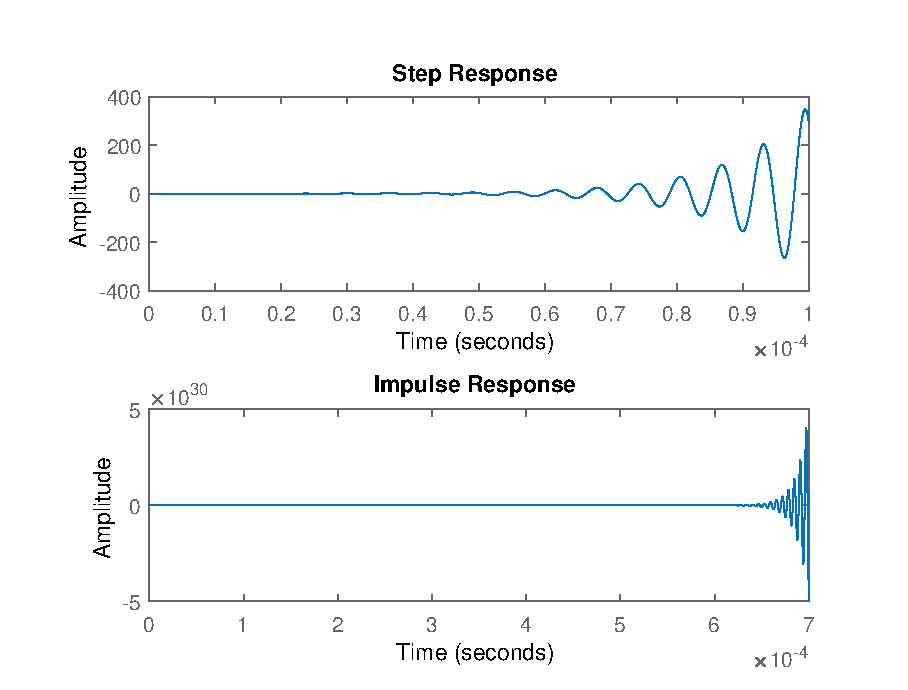
\includegraphics[width=\textwidth]{img/CoilRigResponse.eps}
    \caption{Step and impulse response for $H(j\omega)$}
    \label{fig:step}
\end{figure}

Here we see that we have a damped sinusiodal response with a frequency $f_s$ of 156kHz witch is the same frequency as the resonance frequency $f_0$ of the frequency response. This response attenuates within a few cycles.

\Cref{fig:polezero} shows the poles and zeros of the transfer function $H(j\omega)$ of the resonant circuit.

\begin{figure}[H]
    \centering
    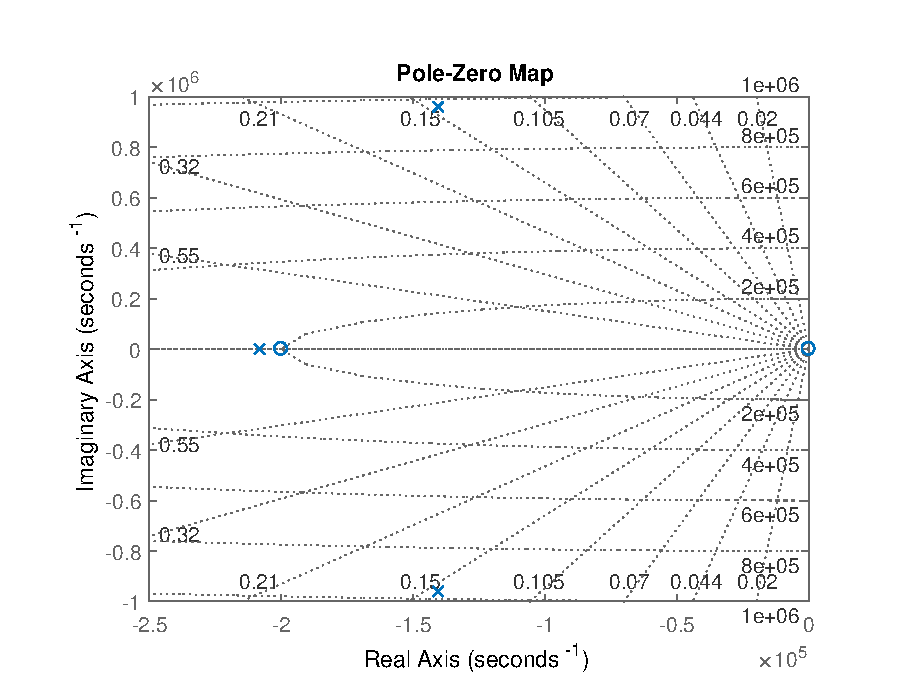
\includegraphics[width=\textwidth]{img/CoilRigPoleZeroPlot.eps}
    \caption{PoleZeroPlot for $H(j\omega)$}
    \label{fig:polezero}
\end{figure}

\Cref{tab:coilrigpoles} shows the numerical values of the poles and zeros of the transfer function $H(j\omega)$ of the resonant circuit.

\begin{table}[h]
    \centering
    \begin{tabular}{c|c}
        Poles & Zeros \\
        $(-1,4 + 9,6i)\cdot 10^{5} s^{-1}$ & $0$ \\
        $(-1,4 - 9,6i)\cdot 10^{5} s^{-1}$ & $0$ \\
        $(-2,1 + 0i)\cdot 10^{5} s^{-1}$ & $-2\cdot 10^{5} s^{-1}$ \\
    \end{tabular}
    \caption{Poles and zeros for $H(j\omega)$}
    \label{tab:coilrigpoles}
\end{table}

Here we observe a pole pair in the left half plane, a single real pole in the left half plane. As well as three zeros, one in the left half plane and two in origo.

\Cref{fig:crlinsim} shows the result of a linear simulation of the transfer function of the resonant circuit with a 160V peak square wave input signal with amplitude 1 and frequency 159kHz.

\begin{figure}[H]
    \centering
    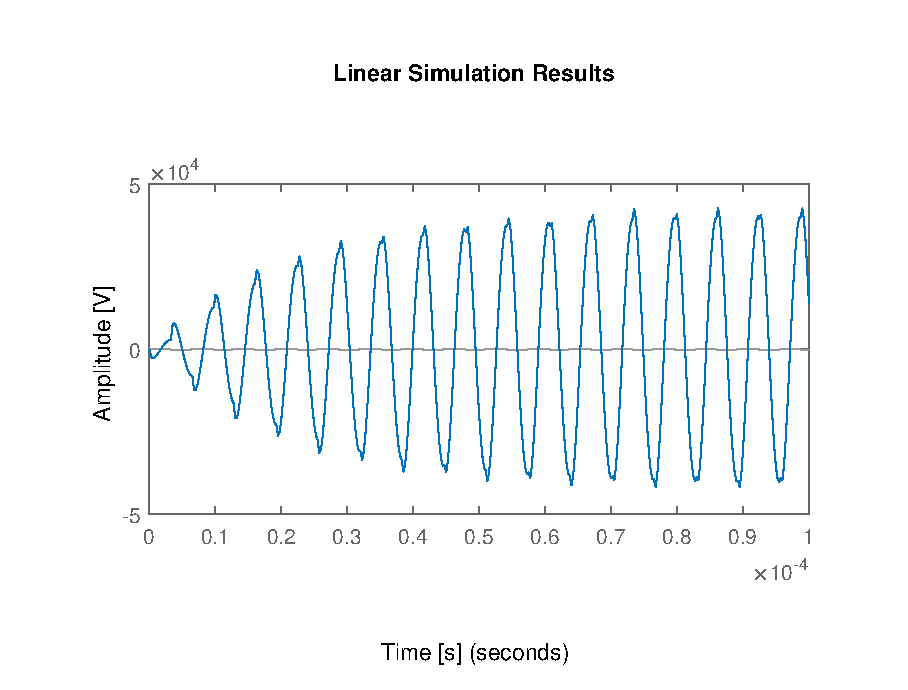
\includegraphics[width=\textwidth]{img/CoilRigSimulation.eps}
    \caption{Linear simulation of transfer function with square wave with $f=f_0$ as input}
    \label{fig:crlinsim}
\end{figure}

We see here that the output signal X6 starts with a quarter period of the step response shown in \cref{fig:step}, and then when the voltage peaks, meaning when the differential of the voltage is zero, a new step response with opposite phase is added to the output signal. This makes the output signal grow rapidly for three cycles to 160kV, before flattening out at 170kV.

\newpage
\section{Transfer function for feedback}
If we use \cref{eq:1} and \cref{eq:2} and solve for $\frac{I_1}{U_{X6}}$ we get the transfer function for the feedback signal shown in \cref{eq:fb_1} to \cref{eq:fb_q}. Where $Z_1$ to $Z_4$ are the same impedances as given in \cref{eq:3_1}.

\begin{equation} \label{eq:fb_1}
\frac{I_1}{U_{X6}} = H_{FB}(s) = \frac{Z_2-Z_3-Z_4}{(Z_1+Z_2)(Z_2-Z_3-Z_4)-Z_2^2}
\end{equation}

\begin{equation} \label{eq:fb_2}
    H_{FB}(s) = \frac{s^3 h + s^2 k + s l}{s^4 m + s^3 n + s^2 o + s p + q}
\end{equation}

Where

\begin{equation}
    h = 2(C_1 C_2 G_1 M) - (C_1 C_2 G_1 L_2)
\end{equation}

\begin{equation}
    k = -(C_1 C_2 G_1 R_2) - (C_1 C_2)
\end{equation}

\begin{equation}
    l = -C_1 G_1
\end{equation}

\begin{equation}
    m = (C_1 C_2 G_1 L_1 L_2)-2(C_1 C_2 G_1 L_1 M)
\end{equation}

\begin{equation} \label{eq:fb_n}
    n = (C_1 C_2 G_1 L_1 R_2) + (C_1 C_2 L_1) + (C_1 C_2 G_1 R_1 L_2) - 2(C_1 C_2 G_1 R_1 M)
\end{equation}

\begin{equation} \label{eq:fb_o}
    o = (C_1 G_1 L_1) + (C_1 C_2 R_1) + (C_2 G_1 L_2) -2(C_2 G_1 M)
\end{equation}

\begin{equation} \label{eq:fb_p}
    p = (C_1 G_1 R_1) + (C_2 G_1 R_2) + C_2
\end{equation}

\begin{equation} \label{eq:fb_q}
    q = G_1
\end{equation}

\Cref{fig:fb_bode} Shows the bode plot for the transfer function $H_{FB}(j\omega)$ for the feedback signals X8 and X9 (both are identical).

\begin{figure}[H]
    \centering
    \includegraphics[width=\textwidth]{img/FeedBackBode.eps}
    \caption{Bode plot of the transfer function for the feedback signals $H_{FB}(j\omega)$}
    \label{fig:fb_bode}
\end{figure}

Here we see a much sharper peak at the resonant frequency than in the bode plot for the resonant circuit $H(j\omega)$. We also see that the response does not flatten at frequencies higher than the resonance frequency. The resonant frequency $f_0$ is 160kHz and the magnitude is 0dB at resonance.


\Cref{fig:fb_step} shows the step and impulse response of the feedback transfer function $H_{FB}(j\omega)$.

\begin{figure}[H]
    \centering
    \includegraphics[width=\textwidth]{img/FeedBackResponse.eps}
    \caption{Step and impulse response of transfer function for the feedback current}
    \label{fig:fb_step}
\end{figure}

Here we see a damped sinusoiodal response with a frequency $f_s$ of 167kHz witch is slightly higher than the resonant frequency $f_0$ of 160kHz. The step response of the feedback signal attenuates slower than the step response of the resonant circuit.

\Cref{fig:fbpolezero} shows the pole and zero plot for the transfer function for the feedback signals $H_{FB}(j\omega)$.

\begin{figure}[H]
    \centering
    \includegraphics[width=\textwidth]{img/FeedBackPoleZeroPlot.eps}
    \caption{PoleZeroPlot for $H_{FB}(j\omega)$}
    \label{fig:fbpolezero}
\end{figure}

\Cref{tab:fbcoilrigpoles} shows the numerical values of the poles and zeros of the transfer function for the feedback signals $H_{FB}(j\omega)$.

\begin{table}[h]
    \centering
    \begin{tabular}{c|c}
        Poles & Zeros \\
        $(-47 + 0i)\cdot 10^{5} s^{-1}$ & \\
        $(-0,5 + 10i)\cdot 10^{5} s^{-1}$ & $0$ \\
        $(-0,5 - 10i)\cdot 10^{5} s^{-1}$ & $-48\cdot 10^{5} s^{-1}$ \\
        $(-2,1 + 0i)\cdot 10^{5} s^{-1}$ & $-2,1\cdot 10^{5} s^{-1}$ \\
    \end{tabular}
    \caption{Poles and zeros for $H_{FB}(j\omega)$}
    \label{tab:fbcoilrigpoles}
\end{table}

Here we observe a pole pair in the left half plane, two real poles in the left half plane. As well as three zeros, two in the left half plane and one in origo.

\Cref{fig:fblinsim} shows the result of a linear simulation of the transfer function of the feedback signal with a 160V peak square wave input signal with amplitude 1 and frequency 159kHz.

\begin{figure}[H]
    \centering
    \includegraphics[width=\textwidth]{img/FeedBackSimulation.eps}
    \caption{Linear simulation of transfer function with square wave with $f=f_0$ as input}
    \label{fig:fblinsim}
\end{figure}

Here we see a sinusoidal current that grows rapidly for 9 cycles to 182A then stabilizes at 186A. We also see that the input signal switches when the current is zero, though after some cycles the input signal drifts out of sync with the current.

\newpage
\section{Magnitude analysis}
By taking the magnitudes for each variable listed in \cref{tab:mod_params} and inserting them into the different terms in the transfer function $H(s)$ (\cref{eq:4}) we can see witch terms influence the result and witch terms are insignificant. In \cref{tab:termsh} the values of each of the terms making up the main terms in \cref{eq:4}, are listed after inserting the magninudes in \cref{tab:mod_params}. e, f, and g are not listed since they only have a single term each.

\begin{table}[H]
    \centering
    \begin{tabular}{c|c|c}
        a & $(C_1 C_2 G_1 L_1 L_2)$   & $2 \cdot 10^{-29}$ \\
          & $2 (C_1 C_2 G_1 L_1 M)$   & $8 \cdot 10^{-32}$ \\
          & $(C_1 C_2 G_1 M^2)$       & $8 \cdot 10^{-31}$ \\
        \hline
        b & $(C_1 C_2 G_1 L_1 R_2)$   & $2 \cdot 10^{-26}$ \\
          & $(C_1 C_2 G_1 L_2 R_1)$   & $2 \cdot 10^{-23}$ \\
          & $2 (C_1 C_2 G_1 M R_1)$   & $8 \cdot 10^{-26}$ \\
          & $(C_1 C_2 L_1)$           & $1 \cdot 10^{-23}$ \\
        \hline
        c & $(C_1 C_2 G_1 R_1 R_2)$   & $2 \cdot 10^{-20}$ \\
          & $(C_1 C_2 R_1)$           & $1 \cdot 10^{-17}$ \\
          & $(C_1 G_1 L_1)$           & $2 \cdot 10^{-17}$ \\
          & $(C_2 G_1 L_2)$           & $2 \cdot 10^{-17}$ \\
          & $2 (C_2 G_1 M)$           & $8 \cdot 10^{-20}$ \\
        \hline
        d & $(C_1 G_1 R_1)$           & $2 \cdot 10^{-11}$ \\
          & $(C_2 G_1 R_2)$           & $2 \cdot 10^{-14}$ \\
          & $C_2$                     & $1 \cdot 10^{-11}$ \\
    \end{tabular}
    \caption{Magnitudes of parameters in H(s)}
    \label{tab:termsh}
\end{table}

From \cref{tab:termsh} we see that the first term of $a$ is the largest, and the second and third terms are two and one orders smaller. Thus they are not significant and can be removed without reducing accuracy significantly. Further the first and third terms of $b$ are three orders smaller than the second and fourth terms and can be removed with the same reasoning. The second and fourth terms of $b$ are of the same magnitude and is thus equally significant. Two terms can be removed from $c$ and one term from $d$. e, f, and g only contains one term each and can not be simplified. This gives the simplified main parameters shown in \cref{eq:ab_simp} and \cref{eq:cd_simp}.

\begin{equation} \label{eq:ab_simp}
    a' = (C_1 C_2 G_1 L_1 L_2), b' = [(C_1 C_2 G_1 L_2 R_1)+(C_1 C_2 L_1)],
\end{equation}
\begin{equation} \label{eq:cd_simp}
    c' = [(C_1 C_2 R_1)+(C_1 G_1 L_1)+(C_2 G_1 L_2)], d' = [(C_1 G_1 R_1) + C_2]
\end{equation}

Inserting the magnitudes from \cref{tab:mod_params} in $H(s)$ both before and after simplifying gives the same result when rounded to one significant digit as shown in \cref{tab:beforeafter}.

\begin{table}[h!]
    \centering
    \begin{tabular}{c|c|c}
          & Before             & After \\ \hline
        a & $2 \cdot 10^{-29}$ & $2 \cdot 10^{-29}$ \\
        b & $3 \cdot 10^{-23}$ & $3 \cdot 10^{-23}$ \\
        c & $5 \cdot 10^{-17}$ & $5 \cdot 10^{-17}$ \\
        d & $3 \cdot 10^{-11}$ & $3 \cdot 10^{-11}$ \\
        e & $2 \cdot 10^{-05}$ & $2 \cdot 10^{-05}$ \\
        f & $2 \cdot 10^{-22}$ & $2 \cdot 10^{-22}$ \\
        g & $4 \cdot 10^{-16}$ & $4 \cdot 10^{-16}$ \\
    \end{tabular}
    \caption{Terms in H(s) before and after magnitude analysis with one significant digit}
    \label{tab:beforeafter}
\end{table}

\todo{a,b,c,d,e,f,og g er alle signifikante. Hvordan bevise?}

\section{Streamer}
\label{sec:arc}

When the electric discharge from the top load of the resonant circuit forms long threads or filaments in the air this is called a streamer discharge \citep{streamer}. When a streamer discharge happens this affects the resonant circuit, this influence is proposed modeled as a varying conductance. A model for this conductance is found from an article \citep{575670} combining two classical models for electric discharge. This model is shown in \cref{eq:g1},

\begin{equation} \label{eq:g1}
    G_1 = G_{min} + [ 1 - \exp(-\frac{i_{G1}^2}{I_0^2})] \frac{U_{X7} i_{G1}}{E_0^2} + [\exp(-\frac{i_{G1}^2}{I_0^2})] \frac{i_{G1}^2}{P_0} - \theta \frac{d G_1}{dt}
\end{equation}

where

\begin{equation}
    \theta = \theta_0 + \theta_1 exp(-\alpha |i|)
\end{equation}

and the parameters in this model are shown in \cref{tab:g1params}.

\begin{table}[h]
    \centering
    \begin{tabular}{c|c|c|c}
         & Comment &  &\\ \hline
        $G_{min}$ & Least possible conductance &  &\\
        $\theta$  & Streamer dampening factor &  &\\
        $I_o$     & Limit between large and small current &  &\\
        $E_0$     & Constant, steady state streamer voltage &  &\\
        $P_0$     & Constant power loss from streamer &  & \\
        $i_{G1}$  & Current flowing in streamer      &  & \\
        $U_{X7}$     & Voltage over streamer            &  &
    \end{tabular}
    \caption{Parameters for model for $G_1$}
    \label{tab:g1params}
\end{table}

$G_{min}$ is the least possible conductance from the top load $C_2$ to ground. This conductance is present before any streamers form as well as after streamers have formed.

\todo{Corona?}

\subsection{Streamer capacitance}
It is also proposed, based on the general consensus in the hobby community \citep{streamercapacitance}, that the streamer increases the capacitance of the top load $C_2$.

\begin{equation}
    C_2' = C_2 + C_s = C_2 + l C_u
\end{equation}

Where $C_s$ is the capacitance introduced by the streamer. $l$ is the length of the streamer in meters, $C_u$ is the capacitance of the streamer per meter. This is an approximation, the actual capacitance of the streamer can be calculated from the definition of capacitance and becomes a complicated equation that also dependts on the ration between length and width of the streamer \citep{thinstraight}. Two values for the capacitance per meter used in the hobby community are 25pF \citep{conner}, and 5pF \citep{scantesla}.

\section{Varying parameters}

\begin{figure}[H]
    \centering
    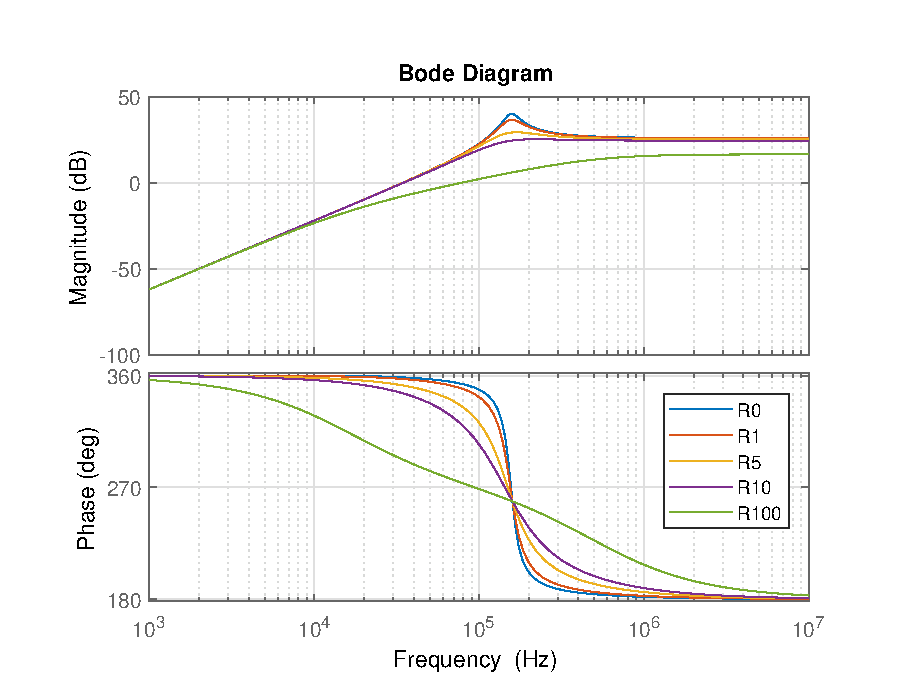
\includegraphics[width=\textwidth]{img/CoilRigBode_R1.eps}
    \caption{Bode plot of $H(j\omega)$ varying R1}
    \label{fig:bode_r1}
\end{figure}

\begin{figure}[H]
    \centering
    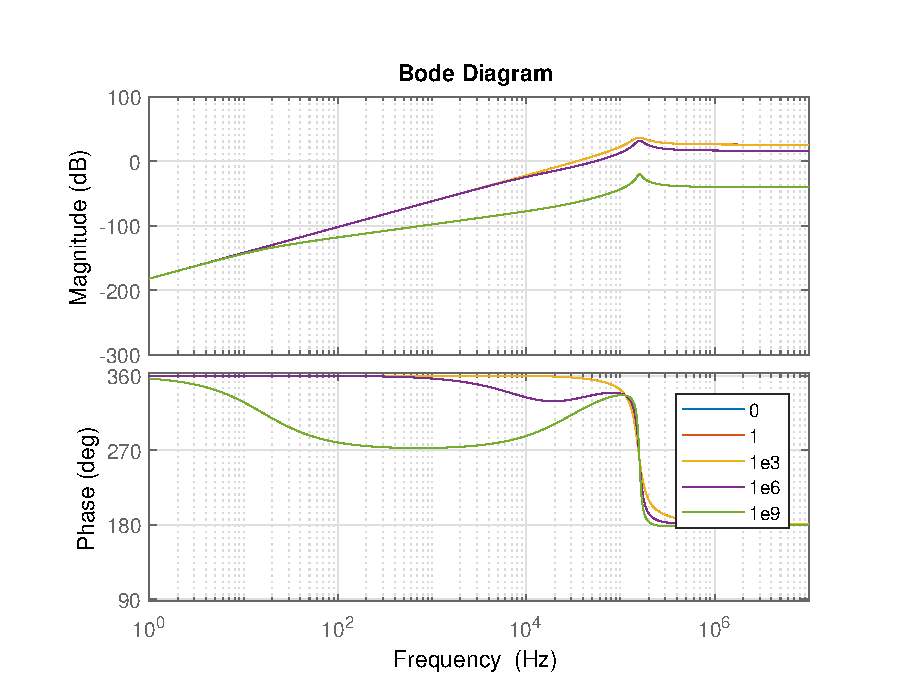
\includegraphics[width=\textwidth]{img/CoilRigBode_R2.eps}
    \caption{Bode plot of $H(j\omega)$ varying R2}
    \label{fig:bode_r2}
\end{figure}

\begin{figure}[H]
    \centering
    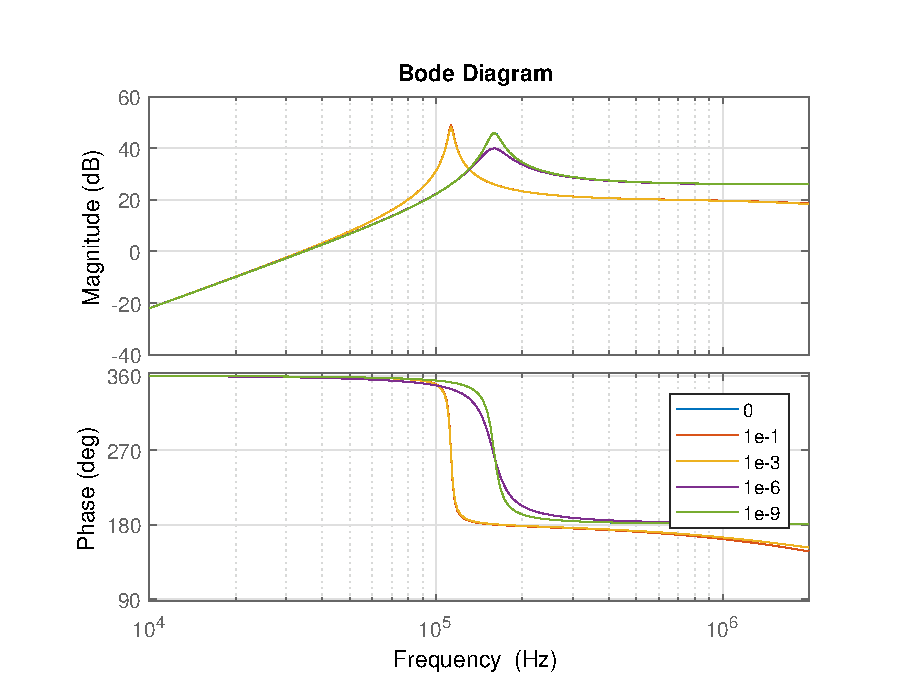
\includegraphics[width=\textwidth]{img/CoilRigBode_G1.eps}
    \caption{Bode plot of $H(j\omega)$ varying G1}
    \label{fig:bode_g1}
\end{figure}

\begin{figure}[H]
    \centering
    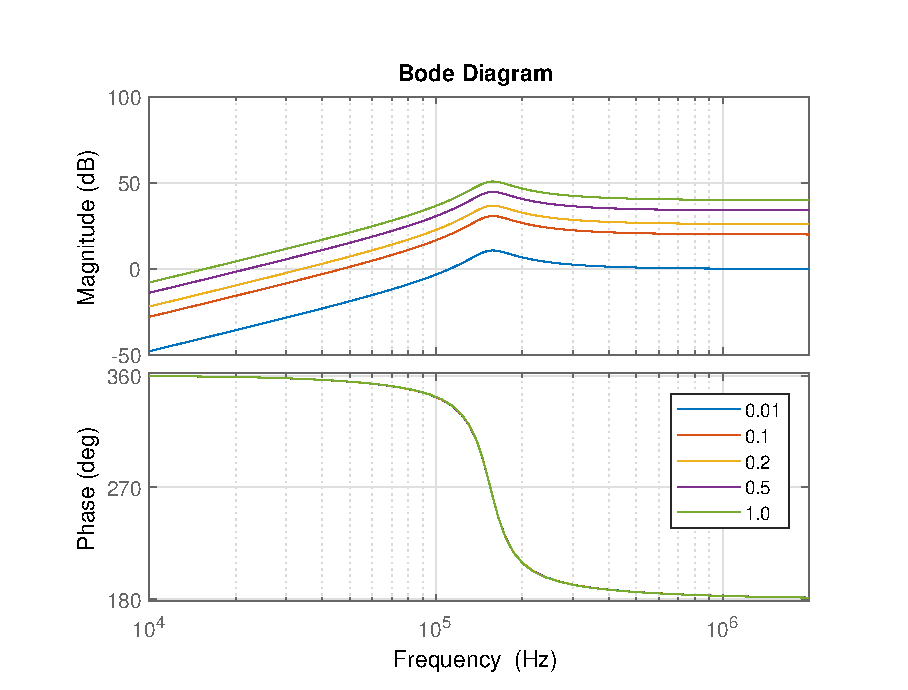
\includegraphics[width=\textwidth]{img/CoilRigBode_k.eps}
    \caption{Bode plot of $H(j\omega)$ varying k}
    \label{fig:bode_k}
\end{figure}

%Målebeskrivelse
\section{Methodology}

\subsection{Acoustic measurements}

%Måleresultater
\chapter{Results}
What are the measurement/model results

\section{Acoustic measurements}

\begin{figure}
    \centering
    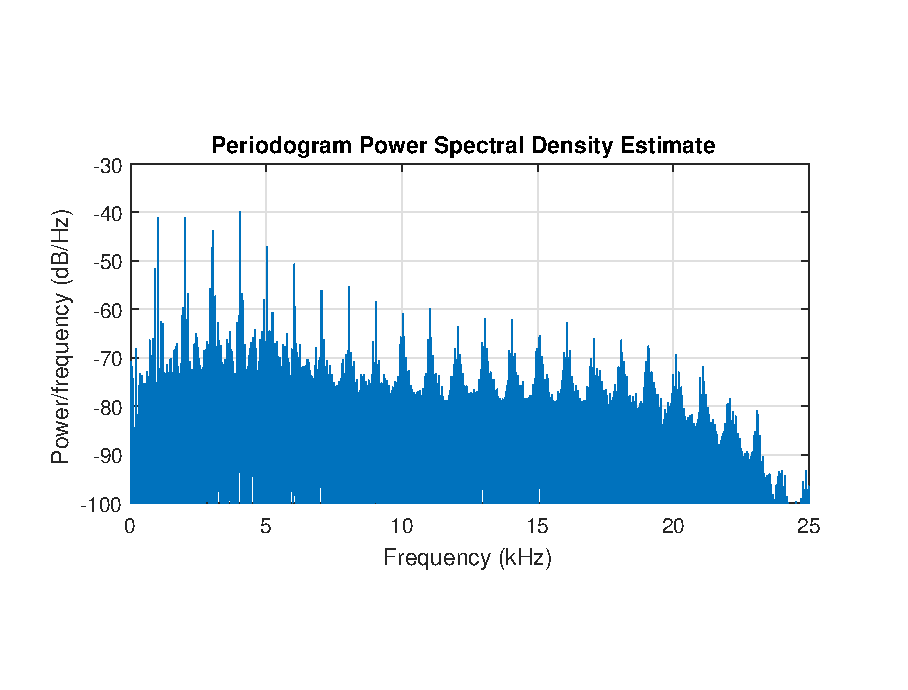
\includegraphics[trim={0cm 1.6cm 0cm 2cm},clip,width=\textwidth]{img/Periodogram_1khz-09.eps}
    \caption{Periodogram of 1kHz recorded tone}
    \label{fig:period_1k}
\end{figure}

\begin{figure}
    \centering
    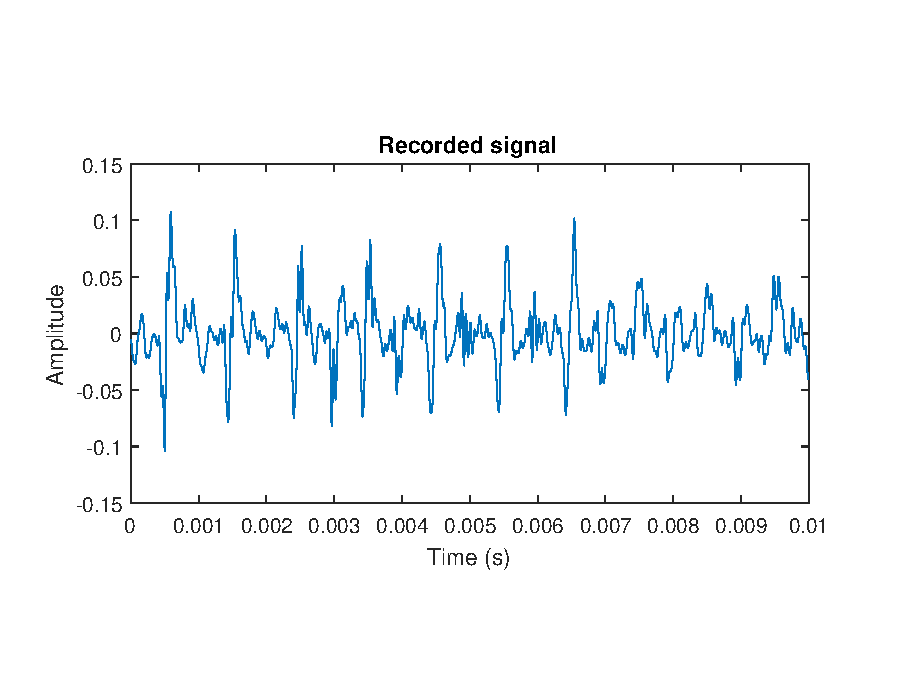
\includegraphics[trim={0cm 1.6cm 0cm 2cm},clip,width=\textwidth]{img/Recorded_1khz-09.eps}
    \caption{Time domain plot of 1kHz recorded tone}
    \label{fig:recorded_1k}
\end{figure}
%Diskusjon
%\chapter{Discussion}
How does the theory and practice fit together, is this acceptable? good enough? Unless done in results

%Konklusjon
\chapter{Conclusion}
It is like this!
%Videre arbeid
\section{Topics for further research}

There is a broad agreement in the hobby community that the streamer affects the system, but its effects on the system are not clear from the work done here. Parameters for the streamer model mentioned should be found to further investigate how the streamer influences the voltages and currents on the output.

The component values and parameters and its effect on the output signal are only substantiated with theoretical work and should be verified experimentally.

By varying the supply voltage for the power amplifier one could acheive AM modulation instead of PDM modulation.

When pulses on the input $X2$ get too close, the coil rig has not had time to swing down, if a new pulse is input before it has swung down one may risk switching while the current is not zero, and the response may be different. It would be interesting to investigate wether the latch in the interrupter will or can be used to keep the signal $X5$ in sync.

%Inngående beskrivelse, analyse og dokumentasjon av en DRSSTC implementasjon.

%Introduksjon
%Beskrivelse av Tesla Coil / DRSSTC
%Tidligere arbeid
%Teori?
%Beskrivelse av arkitektur (Blokkoppbygning)
%Inngående beskrivelse av kretsene (inkludert designvalg)
%Inngående beskrivelse av signaler i kretsene
%Matematisk beskrivelse av så mye som mulig av kretsen(e)
%Målebeskrivelse
%Måleresultater
%Diskusjon
%Konklusjon
%Videre arbeid


\newpage
\bibliographystyle{plain}
\bibliography{ref}

%<<byman
%% Configuration of the header strings for the Appendices
\renewcommand{\chaptermark}[1]{%
  \markboth{\MakeUppercase{\appendixname\ \thechapter}}%
  {\MakeUppercase{#1}}
}
\fancyhead[RE,LO]{}

\appendix
%byman>>
\lstset{language=Matlab,%
    %basicstyle=\color{red},
    breaklines=true,%
    morekeywords={matlab2tikz},
    keywordstyle=\color{blue},%
    morekeywords=[2]{1}, keywordstyle=[2]{\color{black}},
    identifierstyle=\color{black},%
    stringstyle=\color{mylilas},
    commentstyle=\color{mygreen},%
    showstringspaces=false,%without this there will be a symbol in the places where there is a space
    numbers=left,%
    numberstyle={\tiny \color{black}},% size of the numbers
    numbersep=9pt, % this defines how far the numbers are from the text
    emph=[1]{for,end,break},emphstyle=[1]\color{red}, %some words to emphasise
    %emph=[2]{word1,word2}, emphstyle=[2]{style},    
}

\chapter{Matlab code}
\label{sec:appdx:matlab}
\section{Transfer}
\begin{lstlisting}
C1 = 1e-7;
C2 = 1e-11;
L1 = 1e-5;
L2 = 1e-1;
k = 0.2;
M  = k*sqrt(L1*L2); %2e-6;
R1 = 1;
R2 = 1e2;
G1 = 2e-6;

fprintf('Expected resonance frequency:\n');
fprintf('%i Hz\n', 1./(2*pi()*sqrt(C1*L1)));

H1 = trans(C1, C2, L1, L2, M, R1, R2, G1);
%H2 = trans(C1, C2, L1, L2, M, R1, R2, G1);
%H3 = trans(C1, C2, L1, L2, M, R1, R2, G1);
%H4 = trans(C1, C2, L1, L2, M, R1, R2, G1);
%H5 = trans(C1, C2, L1, L2,  M, R1, R2, G1);

figure('Name','L2');
bde1 = bodeplot(H1);%,H2,H3,H4,H5);
setoptions(bde1, 'FreqUnits','Hz','Grid','on','Xlim',[1e4, 2e6]);
%legend('0.01','0.8','1.0','1.2','100','Location','northeast');

[mag, phase, W] = bode(H1);
[val, idx] = max(20*log10(squeeze(mag(1,1,:))));
W = W./(2*pi);
fprintf('Max amplitude:\n');
fprintf('%i dB\n', val);
fprintf('%i Hz\n', W(idx));

figure;
subplot(2,1,1)
step(H1, 2e-5); hold on;
[Y, T] = step(H1, 2e-5);
%findpeaks(Y)
[pks1, locs1] = findpeaks(-Y);
[pks2, locs2] = findpeaks(Y);
stepfrequency = 1./(2*(T(locs2(1))-T(locs1(1))))


subplot(2,1,2)
impulse(H1, 2e-5);

figure;
pzplot(H1);
grid on;
[P, Z] = pzmap(H1)

function H = trans(C1, C2, L1, L2, M, R1, R2, G1)
    a  = ((C1*C2*G1*L1*L2)-2*(C1*C2*G1*L1*M)+(C1*C2*G1*M^2));
    b  = ((C1*C2*G1*L1*R2)+(C1*C2*G1*L2*R1)-2*(C1*C2*G1*M*R1)+(C1*C2*L1));
    c  = ((C1*C2*G1*R1*R2)+(C1*C2*R1)+(C1*G1*L1)+(C2*G1*L2)-2*(C2*G1*M));
    d  = ((C1*G1*R1)+(C2*G1*R2)+C2);
    e  = (G1);
    f  = (-1)*(C1*C2*M);
    g  = (-1)*(C1*G1*M);

    H  = tf([f g 0 0],[a b c d e]);
end

function H = transferCurrent(C1, C2, L1, L2, M, R1, R2, G1)
    a  = 2*(C1*C2*G1*M)-(C1*C2*G1*L2);
    b  = 0-(C1*C2*G1*R2)-(C1*C2);
    c  = 0-(C1*G1);
    d  = 0;
    e  = (C1*C2*G1*L1*L2)-2*(C1*C2*G1*L1*M);
    f  = (C1*C2*G1*L1*R2)+(C1*C2*L1)+(C1*C2*G1*R1*L1)-2*(C1*C2*G1*R1*M);
    g  = (C1*G1*L1)+(C1*C2*R1)+(C2*G1*L2)-2*(C2*G1*M);
    h  = (C1*G1*R1)+(C2*G1*R2)+C2;
    k  = G1;

    H  = tf([a b c d],[e f g h k]);
end
\end{lstlisting}

\newpage
\section{Linear simulation}
\begin{lstlisting}
C1 = 1e-7;
C2 = 1e-11;
L1 = 1e-5;
L2 = 1e-1;
k = 0.2;
M  = k*sqrt(L1*L2); %2e-6;
R1 = 1;
R2 = 1e2;
G1 = 2e-6;
%G1 = 2e-7;

% Time domain parameters
fs = 4e6;       % Sampling frequency
dt = 1/fs;      % Time resolution
T = 1;          % Signal duration
t = 0:dt:T-dt;  % Total duration
N = length(t);  % Number of time samples


f0=1/(2*pi*(sqrt(L1*C1)))
f0_s=1/(2*pi*(sqrt(L2*C2)))
f0=1.57e+05
T0 = (fs/f0);
n = 10;

x2=square(2*pi*f0*t);
x2 = x2*160;
x2 = x2(1:int16(n*T0));
x2 = [x2 zeros(1,(N-length(x2)), 'int16')];

H  =  trans(C1, C2, L1, L2, M, R1, R2, G1);

figure;

lsim(H,x2,t);
axis([0 1.5e-4 -5e4 5e4]);
xlabel('Time [s]');
ylabel('Amplitude [V]');
pbaspect([2 1 1]);
\end{lstlisting}

\section{Limiter filter}
\begin{lstlisting}
R2 = 10;
C3 = 1e9;
n1 = 1;
n2 = 100;

H = tf([R2],[R2*C3 1])

bodeplot(H);
[mag,phase,wout] = bode(H);
\end{lstlisting}

\newpage
\section{Audio plot and synthesis}
\begin{lstlisting}
%% Time domain parameters
fs = 96000;     % Sampling frequency
dt = 1/fs;      % Time resolution
T = 5;          % Signal duration
t = 0:dt:T-dt;  % Total duration
N = length(t);  % Number of time samples

%% Signal generation
envelope = [-41 -41 -44 -40 -47 -51 -55 -55 -58 -60 -60 -64 -62 -62 -65 -62 -66 -66 -67 -70 -72 -80]; % In dB/Hz
envelope = db2mag(envelope);
%envelope = envelope+10;
f0 = 1000;       % fundamental frequency
x = envelope(1)*sin(2*pi*f0*t); % fundamental sinusoid
for i = 2:22
    x = x + envelope(i)*sin(2*pi*f0*i*t);
end

%% Magic
[y,fsy] = audioread('1khz - 09.wav');
y = y(fs*2:fs*7);

%% Generated
figure;
subplot(2,2,1);
plot(psd(spectrum.periodogram,x,'Fs',fs,'NFFT',length(x)));
axis([0 25 -100 -30]);
px = audioplayer(x, fs);
%play(px, [1 (get(px, 'SampleRate') * 3)]);
subplot(2,2,2);
plot(t(1:fs*1e-2), x(1:fs*1e-2));
title('Synthesized signal');
xlabel('Time (s)');
ylabel('Amplitude');
%pause(6);

%% Measured
subplot(2,2,3);
plot(psd(spectrum.periodogram,y,'Fs',fs,'NFFT',length(y)));
axis([0 25 -100 -30]);
py = audioplayer(y, fs);
subplot(2,2,4);
plot(t(1:fs*1e-2), y(1:fs*1e-2));
title('Recorded signal');
xlabel('Time (s)');
ylabel('Amplitude');
%play(py, [1 (get(py, 'SampleRate') * 3)]);

figure;
plot(psd(spectrum.periodogram,y,'Fs',fs,'NFFT',length(y)));
axis([0 25 -100 -30]);
pbaspect([2 1 1])
figure;
plot(t(1:fs*1e-2), y(1:fs*1e-2));
pbaspect([2 1 1]);
title('Recorded signal');
xlabel('Time (s)');
ylabel('Amplitude');
\end{lstlisting}
\chapter{Acoustic measurements}

\newpage
\begin{figure}[H]
    \centering
    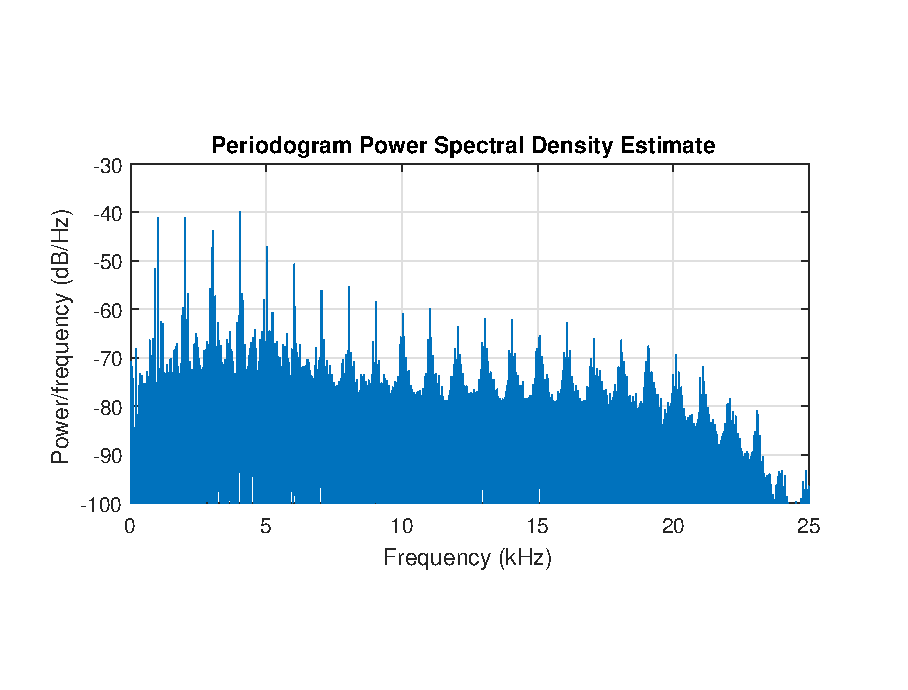
\includegraphics[trim={0cm 1.6cm 0cm 2cm},clip,width=\textwidth]{img/Periodogram_1khz-09.eps}
    \caption{Periodogram of 1kHz recorded tone, duty cycle 09.}
    \label{fig:appdx:period_1k-09}
\end{figure}
\begin{figure}[H]
    \centering
    \includegraphics[trim={0cm 1.6cm 0cm 2cm},clip,width=\textwidth]{img/akustisk/Periodogram_1kHz-10.eps}
    \caption{Periodogram of 1kHz recorded tone, duty cycle 10.}
    \label{fig:appdx:period_1k-10}
\end{figure}

\begin{figure}[H]
    \centering
    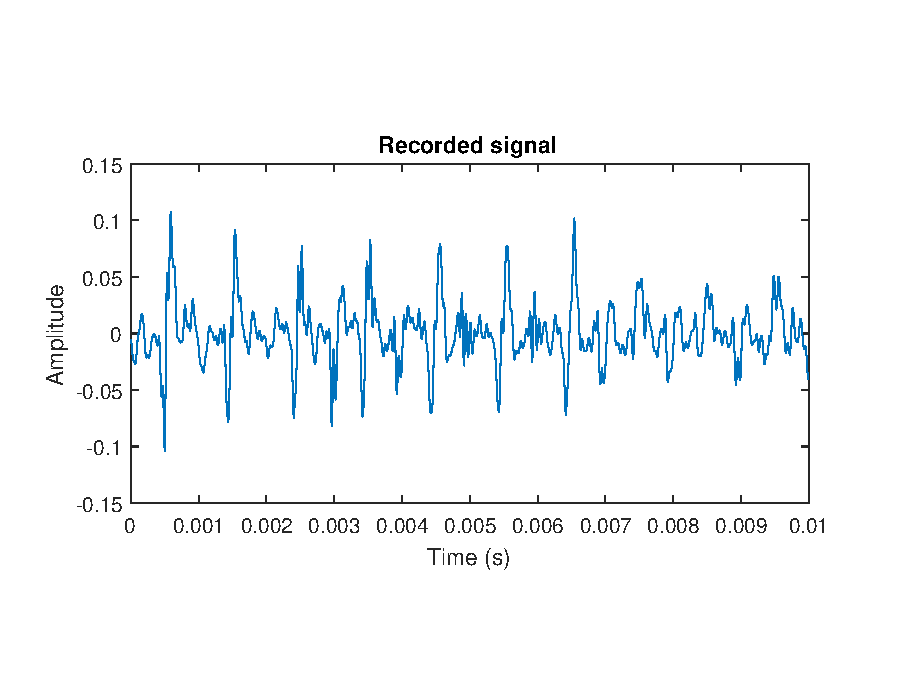
\includegraphics[trim={0cm 1.6cm 0cm 2cm},clip,width=\textwidth]{img/Recorded_1khz-09.eps}
    \caption{Time domain plot of 1kHz recorded tone, duty cycle 09.}
    \label{fig:appdx:wave_1k-09}
\end{figure}
\begin{figure}[H]
    \centering
    \includegraphics[trim={0cm 1.6cm 0cm 2cm},clip,width=\textwidth]{img/akustisk/Waveform_1kHz-10.eps}
    \caption{Time domain plot of 1kHz recorded tone, duty cycle 10.}
    \label{fig:appdx:wave_1k-10}
\end{figure}
%%%%%%%%%%%%%%%%%%%%%%%%%%%%%%%%%%%%%%%%%%%%%%%%%%%%%%%%%%%%%%%%%%%%%%%%%%%%%%%%%%%%%%%%%%%%%%%%%%%%
\begin{figure}[H]
    \centering
    \includegraphics[trim={0cm 1.6cm 0cm 2cm},clip,width=\textwidth]{img/akustisk/Periodogram_250Hz-09.eps}
    \caption{Periodogram of 250Hz recorded tone, duty cycle 09.}
    \label{fig:period_250-09}
\end{figure}
\begin{figure}[H]
    \centering
    \includegraphics[trim={0cm 1.6cm 0cm 2cm},clip,width=\textwidth]{img/akustisk/Periodogram_250Hz-10.eps}
    \caption{Periodogram of 250Hz recorded tone, duty cycle 10.}
    \label{fig:period_250-10}
\end{figure}

\begin{figure}[H]
    \centering
    \includegraphics[trim={0cm 1.6cm 0cm 2cm},clip,width=\textwidth]{img/akustisk/Waveform_250Hz-09.eps}
    \caption{Time domain plot of 250Hz recorded tone, duty cycle 09.}
    \label{fig:appdx:wave_250-09}
\end{figure}
\begin{figure}[H]
    \centering
    \includegraphics[trim={0cm 1.6cm 0cm 2cm},clip,width=\textwidth]{img/akustisk/Waveform_250Hz-10.eps}
    \caption{Time domain plot of 250Hz recorded tone, duty cycle 10.}
    \label{fig:appdx:wave_250-10}
\end{figure}
%%%%%%%%%%%%%%%%%%%%%%%%%%%%%%%%%%%%%%%%%%%%%%%%%%%%%%%%%%%%%%%%%%%%%%%%%%%%%%%%%%%%%%%%%%%%%%%%%%%%
\begin{figure}[H]
    \centering
    \includegraphics[trim={0cm 1.6cm 0cm 2cm},clip,width=\textwidth]{img/akustisk/Periodogram_63Hz-09.eps}
    \caption{Periodogram of 63Hz recorded tone, duty cycle 09.}
    \label{fig:period_63-09}
\end{figure}
\begin{figure}[H]
    \centering
    \includegraphics[trim={0cm 1.6cm 0cm 2cm},clip,width=\textwidth]{img/akustisk/Periodogram_63Hz-10.eps}
    \caption{Periodogram of 63Hz recorded tone, duty cycle 10.}
    \label{fig:period_63-10}
\end{figure}

\begin{figure}[H]
    \centering
    \includegraphics[trim={0cm 1.6cm 0cm 2cm},clip,width=\textwidth]{img/akustisk/Waveform_63Hz-09.eps}
    \caption{Time domain plot of 63Hz recorded tone, duty cycle 09.}
    \label{fig:appdx:wave_63-09}
\end{figure}
\begin{figure}[H]
    \centering
    \includegraphics[trim={0cm 1.6cm 0cm 2cm},clip,width=\textwidth]{img/akustisk/Waveform_63Hz-10.eps}
    \caption{Time domain plot of 63Hz recorded tone, duty cycle 10.}
    \label{fig:appdx:wave_63-10}
\end{figure}
%%%%%%%%%%%%%%%%%%%%%%%%%%%%%%%%%%%%%%%%%%%%%%%%%%%%%%%%%%%%%%%%%%%%%%%%%%%%%%%%%%%%%%%%%%%%%%%%%%%%





\end{document}
